% MigrationBench training-design comparison figure.
% Editable TikZ/LaTeX source; vector PDF output.
% Semantics are frozen in visual_scientific_acceptance_criteria_v1.md.

\documentclass[tikz,border=0pt]{standalone}
\usepackage{tikz}
\usetikzlibrary{arrows.meta,calc}
\usepackage{amsmath,amssymb}
\usepackage{helvet}
\renewcommand{\familydefault}{\sfdefault}

\definecolor{ink}{HTML}{072B45}
\definecolor{arrowblue}{HTML}{156982}
\definecolor{inputblue}{HTML}{0A7FC2}
\definecolor{coordblue}{HTML}{0F6F8F}
\definecolor{hiddenorange}{HTML}{F1A247}
\definecolor{outputviolet}{HTML}{7030A0}
\definecolor{muted}{HTML}{667985}
\definecolor{rulegray}{HTML}{D6E0E5}
\definecolor{softblue}{HTML}{EFF7FB}
\definecolor{softorange}{HTML}{FFF6E8}
\definecolor{softpurple}{HTML}{F6F0FA}

\tikzset{
  mainTitle/.style={font=\sffamily\fontsize{15}{17}\selectfont,align=center,inner sep=0pt},
  subtitle/.style={font=\sffamily\fontsize{8.5}{10}\selectfont,align=center,inner sep=0pt,text=muted},
  stage/.style={font=\sffamily\fontsize{7.6}{9}\selectfont,align=center,inner sep=0pt,text=ink},
  laneTitle/.style={font=\sffamily\fontsize{8.6}{9.8}\selectfont,align=center,inner sep=0pt,text=ink},
  laneSub/.style={font=\sffamily\fontsize{6.6}{7.7}\selectfont,align=center,inner sep=0pt,text=muted},
  body/.style={font=\sffamily\fontsize{7.5}{9}\selectfont,align=center,inner sep=0pt,text=ink},
  small/.style={font=\sffamily\fontsize{6.2}{7.3}\selectfont,align=center,inner sep=0pt,text=muted},
  note/.style={font=\sffamily\fontsize{5.8}{7}\selectfont,align=center,inner sep=0pt,text=muted},
  dataBox/.style={draw=inputblue,fill=softblue,line width=0.9pt,rounded corners=5pt,minimum width=26mm,minimum height=11mm,text width=22mm,font=\sffamily\fontsize{7.3}{8.5}\selectfont,inner sep=2pt},
  initBox/.style={draw=outputviolet,fill=softpurple,line width=0.9pt,rounded corners=5pt,minimum width=23mm,minimum height=11mm,text width=19mm,font=\sffamily\fontsize{7.3}{8.5}\selectfont,inner sep=2pt},
  updateBox/.style={draw=hiddenorange,fill=softorange,line width=0.9pt,rounded corners=5pt,minimum width=24mm,minimum height=11mm,text width=20mm,font=\sffamily\fontsize{7.3}{8.5}\selectfont,inner sep=2pt},
  neutralBox/.style={draw=ink!65,fill=white,line width=0.85pt,rounded corners=5pt,minimum width=24mm,minimum height=11mm,text width=20mm,font=\sffamily\fontsize{7.3}{8.5}\selectfont,inner sep=2pt},
  resultBox/.style={draw=outputviolet,fill=softpurple,line width=0.9pt,rounded corners=5pt,minimum width=27mm,minimum height=11mm,text width=23mm,font=\sffamily\fontsize{7.3}{8.5}\selectfont,inner sep=2pt},
  flow/.style={draw=arrowblue,line width=0.85pt,-{Latex[length=4pt,width=3pt]}},
  provenance/.style={draw=ink!55,dashed,line width=0.65pt,-{Latex[length=3.5pt,width=2.5pt]}},
}

\newcommand{\roleDot}[3]{\fill[#1] (#2,#3) circle (5pt);}
\newcommand{\laneRule}[1]{\draw[rulegray,line width=0.45pt] (25,#1) -- (1575,#1);}

\begin{document}
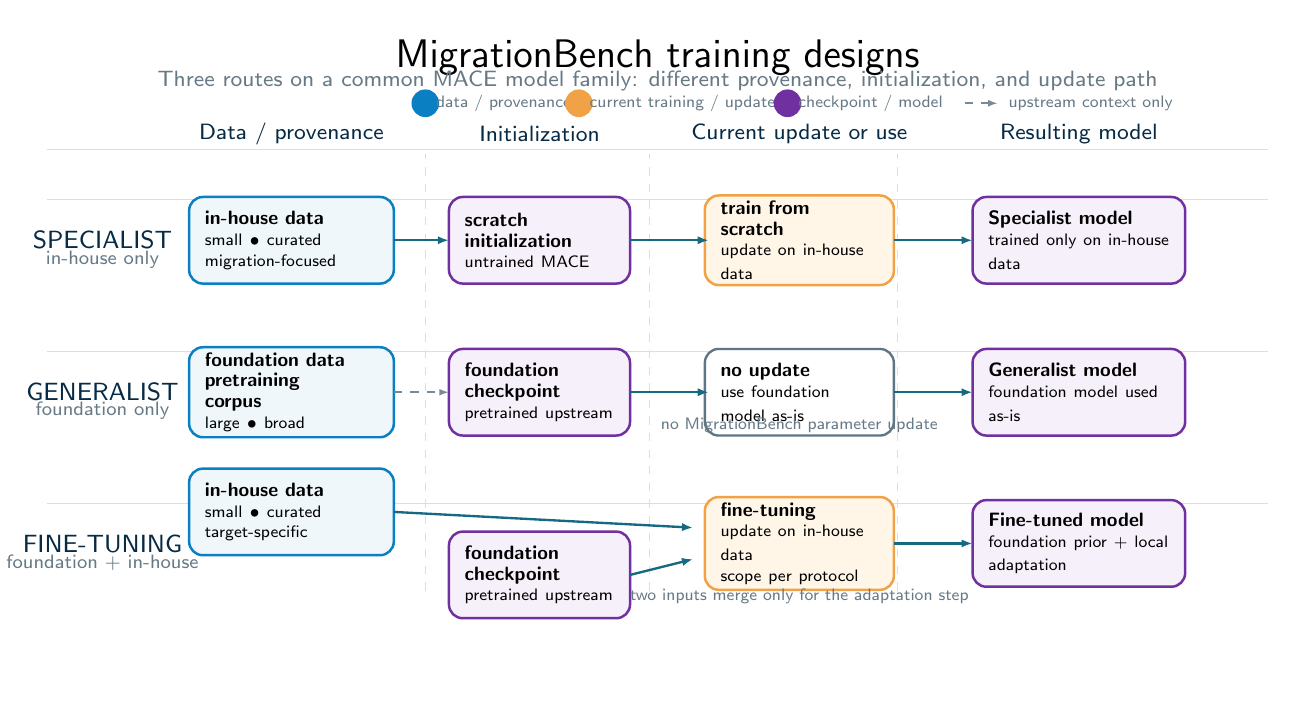
\begin{tikzpicture}[x=0.1mm,y=0.1mm]
  \path[use as bounding box] (0,0) rectangle (1600,820);

  % Neutral title: this is a comparison, not a performance ranking.
  \node[mainTitle] at (800,782) {MigrationBench training designs};
  \node[subtitle] at (800,752) {Three routes on a common MACE model family: different provenance, initialization, and update path};

  % Compact visual legend.
  \roleDot{inputblue}{505}{724}
  \node[small,anchor=west] at (518,724) {data / provenance};
  \roleDot{hiddenorange}{700}{724}
  \node[small,anchor=west] at (713,724) {current training / update};
  \roleDot{outputviolet}{965}{724}
  \node[small,anchor=west] at (978,724) {checkpoint / model};
  \draw[provenance] (1190,724) -- (1232,724);
  \node[small,anchor=west] at (1245,724) {upstream context only};

  % Stage headers and subtle alignment guides.
  \node[stage] at (335,685) {Data / provenance};
  \node[stage] at (650,685) {Initialization};
  \node[stage] at (980,685) {Current update or use};
  \node[stage] at (1335,685) {Resulting model};
  \draw[rulegray,line width=0.35pt] (25,665) -- (1575,665);
  \foreach \x in {505,790,1105} {\draw[rulegray,dashed,line width=0.3pt] (\x,105) -- (\x,660);}

  % Three equal lanes.
  \laneRule{602}
  \laneRule{409}
  \laneRule{216}

  % Lane labels. Their order is layout only; no performance ranking is implied.
  \node[laneTitle] at (95,550) {SPECIALIST};
  \node[laneSub] at (95,526) {in-house only};
  \node[laneTitle] at (95,357) {GENERALIST};
  \node[laneSub] at (95,333) {foundation only};
  \node[laneTitle] at (95,164) {FINE-TUNING};
  \node[laneSub] at (95,140) {foundation + in-house};

  % Specialist: small, curated in-house data -> scratch initialization -> current training -> model.
  \node[dataBox] (sdata) at (335,550) {\textbf{in-house data}\\[-1pt]{\fontsize{6.2}{7.2}\selectfont small $\bullet$ curated}\\[-1pt]{\fontsize{6.2}{7.2}\selectfont migration-focused}};
  \node[initBox] (sinit) at (650,550) {\textbf{scratch}\\[-1pt]\textbf{initialization}\\[-1pt]{\fontsize{6.2}{7.2}\selectfont untrained MACE}};
  \node[updateBox] (supd) at (980,550) {\textbf{train from}\\[-1pt]\textbf{scratch}\\[-1pt]{\fontsize{6.2}{7.2}\selectfont update on in-house data}};
  \node[resultBox] (sout) at (1335,550) {\textbf{Specialist model}\\[-1pt]{\fontsize{6.2}{7.2}\selectfont trained only on in-house data}};
  \draw[flow] (465,550) -- (535,550);
  \draw[flow] (765,550) -- (865,550);
  \draw[flow] (1100,550) -- (1200,550);

  % Generalist: broad upstream data -> foundation checkpoint -> no current update -> model used as-is.
  \node[dataBox] (gdata) at (335,357) {\textbf{foundation data}\\[-1pt]\textbf{pretraining}\\[-1pt]\textbf{corpus}\\[-1pt]{\fontsize{6.2}{7.2}\selectfont large $\bullet$ broad}};
  \node[initBox] (ginit) at (650,357) {\textbf{foundation}\\[-1pt]\textbf{checkpoint}\\[-1pt]{\fontsize{6.2}{7.2}\selectfont pretrained upstream}};
  \node[neutralBox] (guse) at (980,357) {\textbf{no update}\\[-1pt]{\fontsize{6.2}{7.2}\selectfont use foundation model as-is}};
  \node[resultBox] (gout) at (1335,357) {\textbf{Generalist model}\\[-1pt]{\fontsize{6.2}{7.2}\selectfont foundation model used as-is}};
  \draw[provenance] (465,357) -- (535,357);
  \draw[flow] (765,357) -- (865,357);
  \draw[flow] (1100,357) -- (1200,357);

  % Fine-tuning: checkpoint and in-house data are visibly separate inputs that merge only at update.
  \node[dataBox] (fdata) at (335,205) {\textbf{in-house data}\\[-1pt]{\fontsize{6.2}{7.2}\selectfont small $\bullet$ curated}\\[-1pt]{\fontsize{6.2}{7.2}\selectfont target-specific}};
  \node[initBox] (finit) at (650,125) {\textbf{foundation}\\[-1pt]\textbf{checkpoint}\\[-1pt]{\fontsize{6.2}{7.2}\selectfont pretrained upstream}};
  \node[updateBox] (fupd) at (980,165) {\textbf{fine-tuning}\\[-1pt]{\fontsize{6.2}{7.2}\selectfont update on in-house data}\\[-1pt]{\fontsize{6.2}{7.2}\selectfont scope per protocol}};
  \node[resultBox] (fout) at (1335,165) {\textbf{Fine-tuned model}\\[-1pt]{\fontsize{6.2}{7.2}\selectfont foundation prior + local adaptation}};
  \draw[flow] (465,205) -- (845,185);
  \draw[flow] (765,125) -- (845,145);
  \draw[flow] (1100,165) -- (1200,165);

  % Small semantic notes make the non-training Generalist path explicit without adding claims.
  \node[note] at (980,315) {no MigrationBench parameter update};
  \node[note] at (980,98) {two inputs merge only for the adaptation step};
\end{tikzpicture}
\end{document}
